\vspace{-.15in}\section{Research Plan and Methodology}
\label{sec:rep}\vspace{-.075in}

This \xxx project strenghens the reliability of datacenter computing with a 
holistic, thorough methodology. To this end, this section first proposes a 
fast, scalable consensus protocol (\S\ref{sec:protocol}). With this protocol, 
it presents a scheduler that makes general applications fault-tolerant 
(\S\ref{sec:scheduler}) and a new VM replication architecture (\S\ref{sec:vm}). 
The first two objectives include preliminary results. Finally, this section 
describes our research plan (\S\ref{sec:plan}).

\vspace{-.15in}\subsection{Objective 1: Building Fast, Scalable Consensus via
RDMA} 
\label{sec:model}\vspace{-.075in}

% P1: as mentioned in background, a key reason is thread interleavings, 
% so we need to reason about the general patterns we have. Or we say our 
% methodology is just like pattern matching.
Traditional \paxos protocols incur high consensus latency because they run on 
TCP/IP, which go through OS kernels and software network layers. In this 
section, \S\ref{sec:problem} analyzes this latency problem and its poor 
scalability in detail, and then presents our new RDMA-based \paxos 
protocol called \falcon (\S\ref{sec:falcon}).

\vspace{-.15in}\subsubsection{Problem: Consensus Latency of existing \paxos 
protocols scale poorly} 
\label{sec:examples}\vspace{-.075in}

% First, mainly introduce the problems in traditional protocols.
Due to the strong fault-tolerance of \paxos, it is widely served in many 
systems. For instance, Scatter~\cite{scatter:sosp11} runs 8$\sim$12 replicas in 
each \paxos group to order client requests, and it lets replicas respond 
requests in parallel. A bigger group size will improve Scatter throughput. 
Moreover, recent state machine replication (SMR) 
systems~\cite{eve:osdi12,rex:eurosys14,crane:sosp15} use \paxos to greatly 
improve the availability of
general server programs.

Unfortunately, despite these great advances, the high consensus latency of 
\paxos makes systems suffer. For efficiency, \paxos typically assigns one 
replica as the leader to invoke consensus requests, and the other replicas as 
backups to agree on requests. To agree on an input, at least one message 
round-trip is required between the leader and a backup. A round-trip causes big 
latency as it goes through TCP/IP layers such as software network stack and OS 
kernel. This latency could be acceptable for leader 
election~\cite{chubby:osdi,zookeeper} or
heavyweight transactions~\cite{crane:sosp15,eve:osdi12}, but undesirable for
key-value stores~\cite{redis,memcached}.

As replica group size increases, \paxos consensus latency often increases
drastically~\cite{scatter:sosp11} due to the linearly increasing number of 
consensus messages. One common approach to improve \paxos scalability is 
leveraging parallel techniques such as multithreading~\cite{zookeeper, 
spaxos:srds12} or asynchronous IO~\cite{crane:sosp15, libpaxos}. However, the 
high TCP/IP round-trip latency still exists, and synchronizations in these 
techniques frequently invoke expensive OS events such as context switches. We 
ran four \paxos-like protocols~\cite{zookeeper, spaxos:srds12, crane:sosp15, 
libpaxos} on 40Gbps network with only one client sending consensus requests. We 
found that, when replica group size increased from 3 to 9, the consensus 
latency of three protocols increased by \tradlatencyincreaselow to 
\tradlatencyincreasehigh, and \systemcostlow to \systemcosthigh of the increase 
was in OS kernel.

% Second, briefly mention the problem in DARE. and its scalability bottleneck.
As RDMA becomes increasingly popular and cheap, it becomes a promising approach 
to address the \paxos scalability problem. However, due to the unrich RDMA 
operation types, fully exploiting RDMA speed in software systems is widely 
considered challenging by the community~\cite{pilaf:usenix14,herd:sigcomm14,
farm:sosp15,dare:hpdc15}. For instance, \dare~\cite{dare:hpdc15} presents a
two-round, RDMA-based \paxos protocol in a sole-leader manner: leader does all 
RDMA workloads and backups do nothing. \dare was fast with 3 or 5 
replicas. However, our evaluation shows that, as replica group grows, the 
leader met scalability bottlenecks (\eg, polling ACKs). \dare's consensus 
latency increased by \darescalability as the group grows by 35x
(\S\ref{sec:eval-dare}).

\vspace{-.15in}\subsubsection{Falcon: a fast, scalable RDMA-based \paxos 
protocol} 
\label{sec:falcon}\vspace{-.075in}

Our key observation is that we should carefully separate RDMA workloads among
the leader and backups, especially in a scalability-sensitive context. 
Intuitively, we can let both leader and backups do RDMA writes directly on 
destination replicas' memory, and let all replicas poll their local memory to 
receive messages.

Although doing so will consume more CPU resources than a sole-leader 
protocol~\cite{dare:hpdc15}, it has three major benefits. First, the leader 
has less workloads. Second, both leader and backups participate in consensus, 
which makes it possible to reach consensus with only one 
round~\cite{paxos:practical}. Third, all replicas can get rid of 
the expensive RDMA ACK polling and just receive consensus messages on their 
bare, local memory. An analogy is threads receiving other threads' data via 
bare memory, a fast and scalable computation pattern.

We present \xxx,\footnote{We name our system after
falcon, one of the fastest birds.} a new RDMA-based \paxos protocol and its
runtime system. In \xxx, all replicas directly write to destination
replicas' memory and poll messages from local memory to receive messages, and 
our runtime system handles other technical challenges such as message 
atomicity (\S\ref{sec:normal}), efficient input logging (\S\ref{sec:logging}), 
and failure recovery (\S\ref{sec:checkpoint}).

Inheritated from our general SMR system \crane~\cite{crane:sosp15}, \xxx's 
design supports general, unmodified server programs. Within \xxx, a program 
runs as is. \xxx automatically deploys this program on replicas, intercepts 
inputs from a server program's inbound socket calls (\eg, \recv) with a Linux 
technique called LD\_PRELOAD, and invokes its \paxos protocol to enforce same 
inputs across replicas.

% Three figures. First, falcon arch. Second, consensus protocol. Third, falcon 
% results compared to traditional ones and DARE.

\begin{figure}[!htb]
    \begin{minipage}{.49\textwidth}
        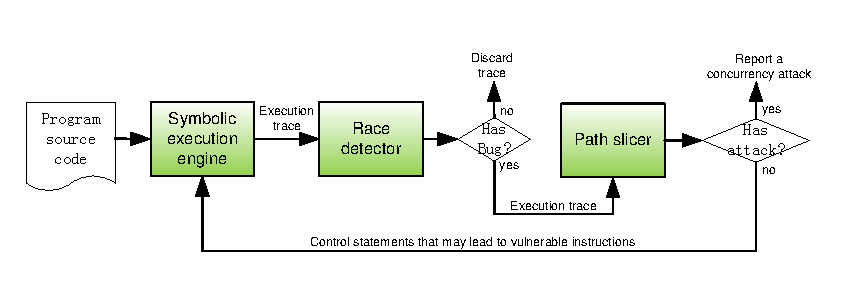
\includegraphics[width=0.34\textheight]{figures/detection}
        \vspace{0.1in}
        \caption{Workflow of detection approach. \\Three basic building blocks
are shaded.}
        \label{fig:falcon-arch}
    \end{minipage}
    \begin{minipage}{0.51\textwidth}
        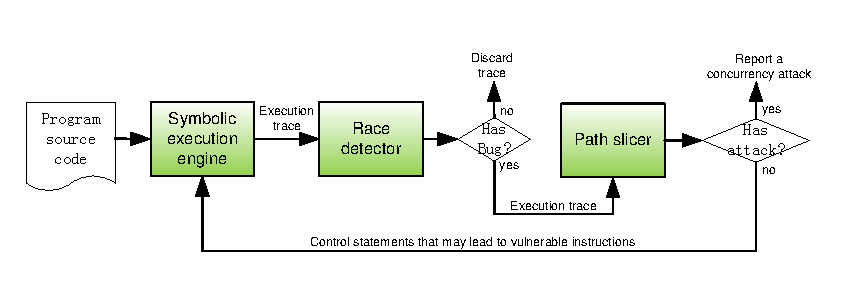
\includegraphics[width=0.34\textheight]{figures/detection}
        \vspace{0.1in}
        \caption{Workflow of detection approach. \\Three basic building blocks
are shaded.}
        \label{fig:falcon-protocol}
    \end{minipage}
\end{figure}

Primilinary results: Crane. Falcon. Say Crane is first version. Falcon totally 
subsumes Crane. Falcon also has initial results.

\vspace{-.15in}\subsection{Objective 2: 
Integrating Falcon with Datacenter Schedulers}\label{sec:detect}\vspace{-.075in}

\vspace{-.15in}\subsubsection{\tripod: the fault-tolerant scheduler 
architecture} 
\label{sec:scheduler-arch}\vspace{-.075in}

TBD.


\vspace{-.15in}\subsubsection{The replication-aware resource allocation scheme}
\label{sec:detect-arch}\vspace{-.075in}

TBD.

Two figures: one is TRIPOD arch. The other is TRIPOD results from the workshop 
paper.

\para{Preliminary results.} Workshop paper.

\para{Future work.} New algorithm on scheduling and replication. Others?

\vspace{-.15in}\subsection{Objective 3: 
Strenghening VM to improve application 
availability}\label{sec:defense}\vspace{-.075in}


% TBD: need a new replication approach name.
\vspace{-.15in}\subsubsection{Idea I: Hybrid Replication} 
\label{sec:defense-arch}\vspace{-.075in}

TBD.

\vspace{-.15in}\subsubsection{Idea II: \paxos-based Live Migration} 
\label{sec:defense-arch}\vspace{-.075in}

TBD.

\vspace{-.15in}\subsection{Research Plan} \label{sec:plan}\vspace{-.075in}

This project will require two PhD students S1 and S2 to work for 
three years. In the first year, S1 will develop and refine the concurrency 
attack model (part of \textbf{Objective~1}), and S2 will leverage the model to 
design the detailed workflow of the detection approach (part of 
\textbf{Objective~2}) by working closely with S1. In the second year, S1 will 
do an empirical study on how well the model represents real-world concurrency 
attacks (part of \textbf{Objective~1}), and S2 will implement the detection 
approach as a software tool (part of \textbf{Objective~2}). In the third year, 
S1 will implement the defense infrastructure (\textbf{Objective~3}), and S2 
will study the detection tool on a broad range of real-world multithreaded 
programs to find new attacks.
% Both students will 
% involve theoretical methods, implement real software systems, and 
% perform real-world study.
% The PI will supervise the students by providing 
% advice concerning both theoretical and systems implementation levels.


